\section{Experimental evaluation}
We evaluated the above mentioned greedy heuristics-based approach in Apache Spark. Spark's SQL optimizer allows passing the optimizer rules externally to the application. We implemented an optimizer that takes the optimized plan as input and based on the heuristics proposed, reorders the joins wherever applicable. It is assumed that the table sizes are available in the Spark optimized plan before applying this rule. We used the TPC DS dataset (scale 100) non-partitioned dataset for evaluating the performance. The experiments were run on a 5 node Apache Spark cluster on AWS with machine type r4.4xlarge.

Out of 100 TPC-DS queries, at least one join in the 38 queries was reordered. We saw on average  For the queries not reordered, the performance would be the same as before. We saw approximately 26\% improvement in the reordered queries and no performance degradation in any of the reordered query. Figure \ref{performance_number}. shows the runtime of a few of the reordered queries.

\begin{figure}[ht]
    \centerline{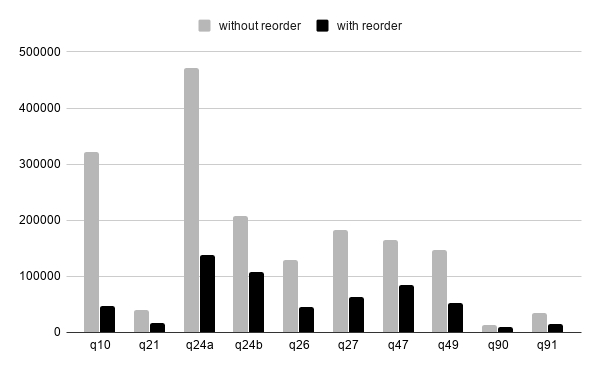
\includegraphics[width=7cm]{fig/chart.png}}
    \caption{Performance reordered sample queries}
    \label{performance_number}
\end{figure}

Out of all reordered queries, 71.1\% reordered queries showed up to 30\% improvement, 15.8\% queries showed between 30 to 60\% improvement and 13.2\% queries showed greater than 60\% improvement.

\begin{figure}[ht]
\centerline{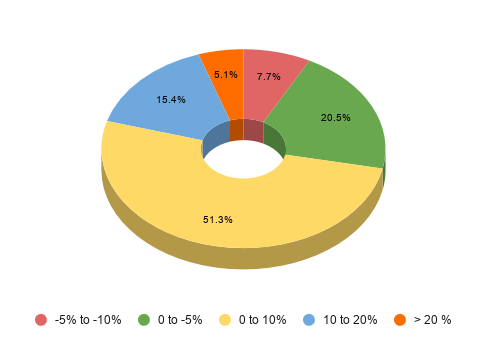
\includegraphics[width=7cm]{fig/pie.png}}
\caption{Improvement the query performance}
\label{performance_pie_chart}
\end{figure}

Let's consider query 21 of TPC-DS benchmark. An oversimplified query plan for the query is depicted in Figure \ref{without-reorder}. The join order in the plan is the same as one given in the query. \texttt{inventory} table first joins with the \texttt{warehouse} table. The result is then joined with \texttt{item} and \texttt{date\_dim} tables respectively

\begin{figure}[ht]
\centerline{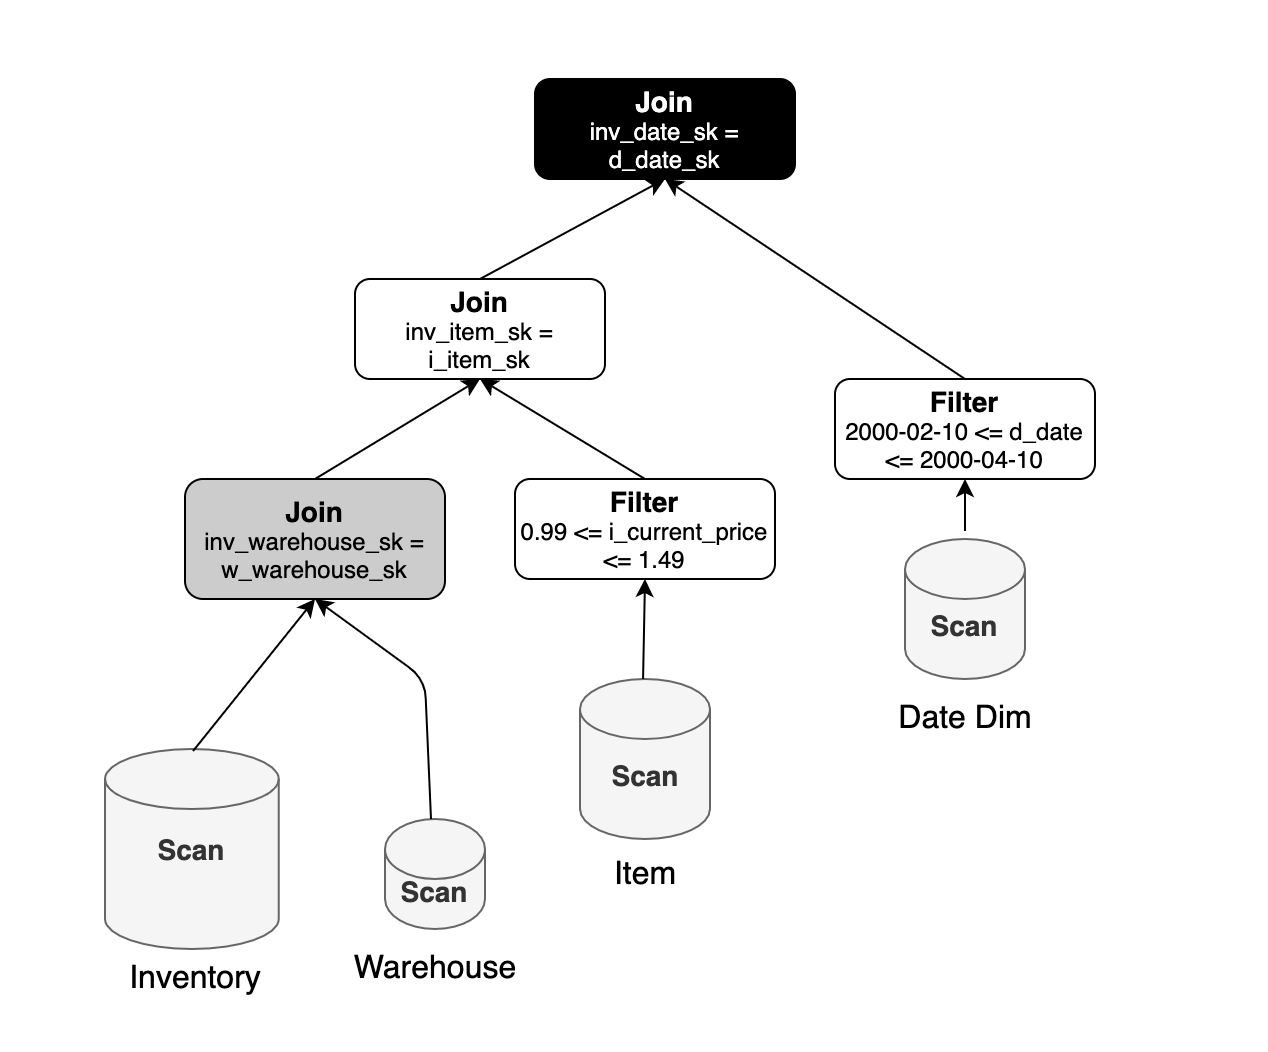
\includegraphics[width=7cm]{fig/without-reorder.png}}
\caption{Query 21 user order}
\label{without-reorder}
\end{figure}

Initially, we extract all consecutive joins from the query plan such that there is only a Project between the two Joins. Once we have the plans of left & right sub-tree and join conditions for each join we try to detect if they form a star schema join. Table \texttt{inventory} is part of the of all three join conditions. So it becomes a candidate for being the fact table and all other tables as dimensions table. Of all the relations referred in the query, \texttt{inventory} table has the largest size followed by \texttt{item}, \texttt{date\_dim} and \texttt{warehouse} respectively. Also the ratio of size of the largest dimensions table \texttt{item} to the fact table candidate, \texttt{inventory} is 0.008, which is lesser than pre-decided configurable threshold of 0.3. Also, none of the dimension tables is partitioned. So based on these heuristics table, we identify the plan has star-schema join with \texttt{inventory} as the fact table and all others as the dimensions table.

After having identified the star schema joins in the query plan, we check that there are no materialize nodes like UDFs and Explode between the scan to ensure that the sizes at the join will be less than or equal to the size at the scan. In the example above, there are only \texttt{Project} and \texttt{Filter} nodes between the scans of tables and all the joins. Also, all the joins are of type \texttt{Inner}. So this example satisfied all the constraints for the Join Reorder and we proceed to reorder the joins if applicable.

Join reorder builds the left deep tree of the joins and constructs them in a bottom-up manner. While building the first join, the plan involving the scan of the identified fact table is selected as the left subtree of the join and right subtree will be chosen from the plans of dimensions table scans. At first, we filter all the plans which have a selective predicate on top of the scan of the dimensions table. If no plan had a selective predicate, we would have taken the plan referred first in the user order. Since in this case, plans corresponding to the scans of \texttt{item} and \texttt{date\_dim} table have a selective predicate, these two plans will be chosen as the potential candidates. Since the table \texttt{date\_dim} has a smaller size, the corresponding plan will be chosen as the right subtree of the first level of the join to be constructed.

In the next steps, a join constructed in the previous step, \texttt{inventory Join date\_dim} in our case will serve as the left subtree of the join to be constructed in this step. The right subtree would be constructed in a similar to the previous step, where it would be picked from the plans corresponding to the available dimensions table scan. Since only the plan corresponding to the scans of \texttt{item} has a selective predicate, it will be chosen as a subtree for creating the second level of the join. In the last step, the plan of the only remaining dimensions table, \texttt{warehouse} will be the last join of the last joins. This procedure is recursively applied until all the dimensions tables are exhausted. Figure \ref{with-reorder} shows the reordered query plan.

\begin{figure}[ht]
\centerline{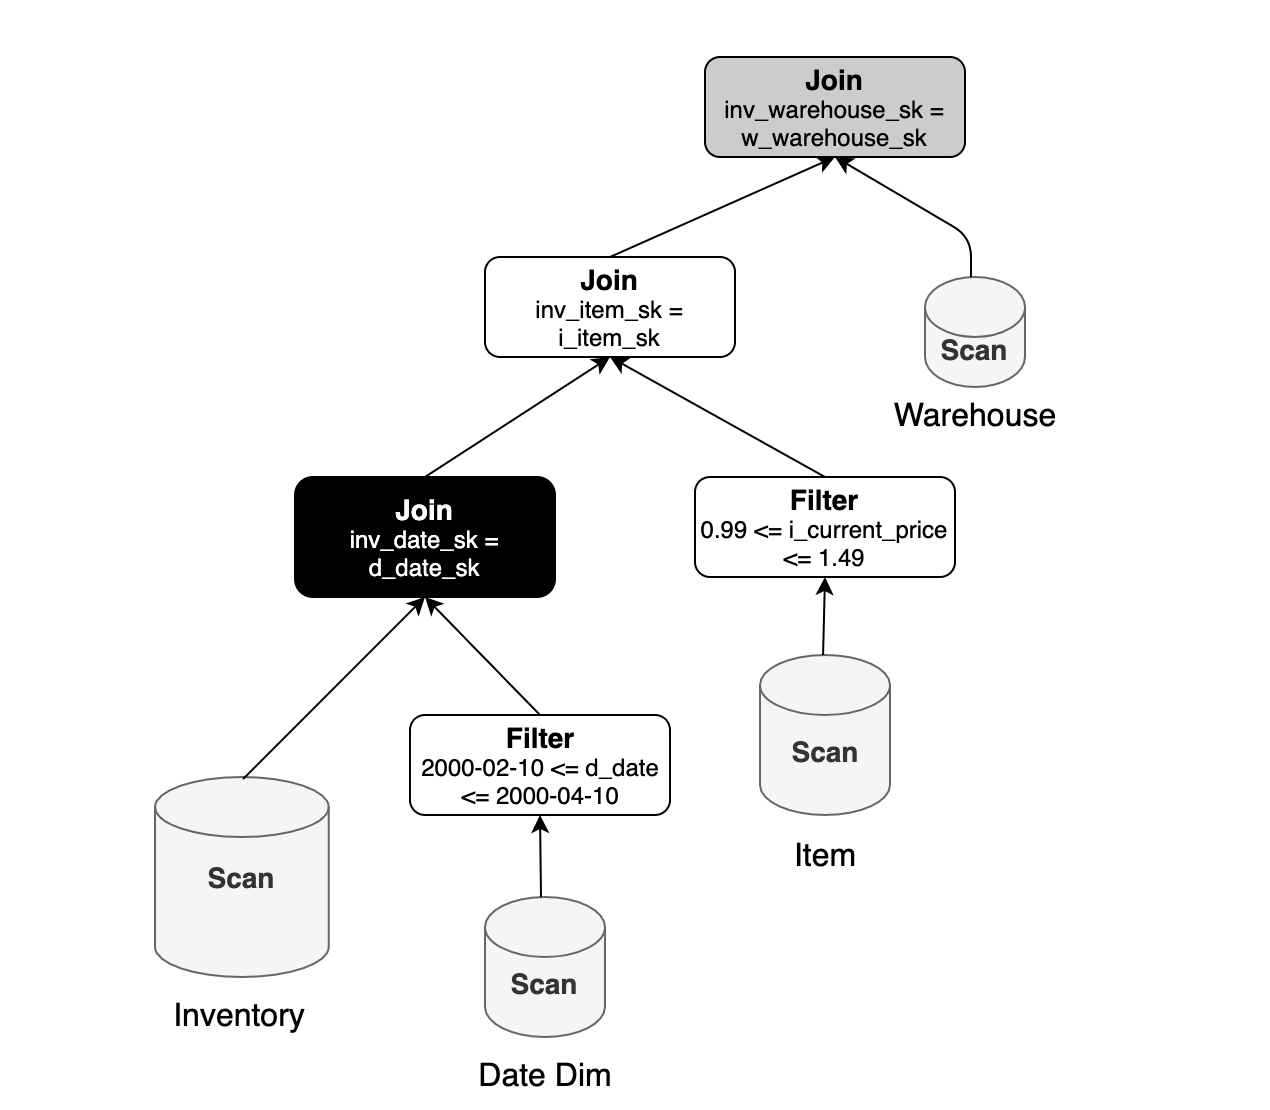
\includegraphics[width=7cm]{fig/with-reorder.png}}
\caption{Query 21 reordered}
\label{with-reorder}
\end{figure}